\chapter{角动量}\label{ch:b1:angular-momentum}

张开双臂旋转的花样滑冰运动员收拢双臂，
无需任何人推动，转速便提高到原来的两倍。
门在把手处一指即可推动，在合页处即便用肩也难以推开。
行星在相等时间内扫过相等的面积——
开普勒在四百年前便已注意到，那时还无人能说明其原因。
月球受自身引起的潮汐作用，每年约以几厘米的速度远离地球，
与此同时，我们的日长也在不知不觉中缓慢增加。
这四种现象背后，都有一个矢量量——\omterm{def:b1:angular-momentum:L}{角动量}，以及一条定律：\omterm{def:b1:angular-momentum:L}{角动量}的变化率等于外\omterm{def:b1:angular-momentum:moment}{力矩}。
本章将定义这两个量，
对质点和质点系证明该定律，
并将其用于\omterm{ex:b1:newton-dynamics:pendulum}{单摆}、轨道和转动物体的分析。

\begin{omfigure}
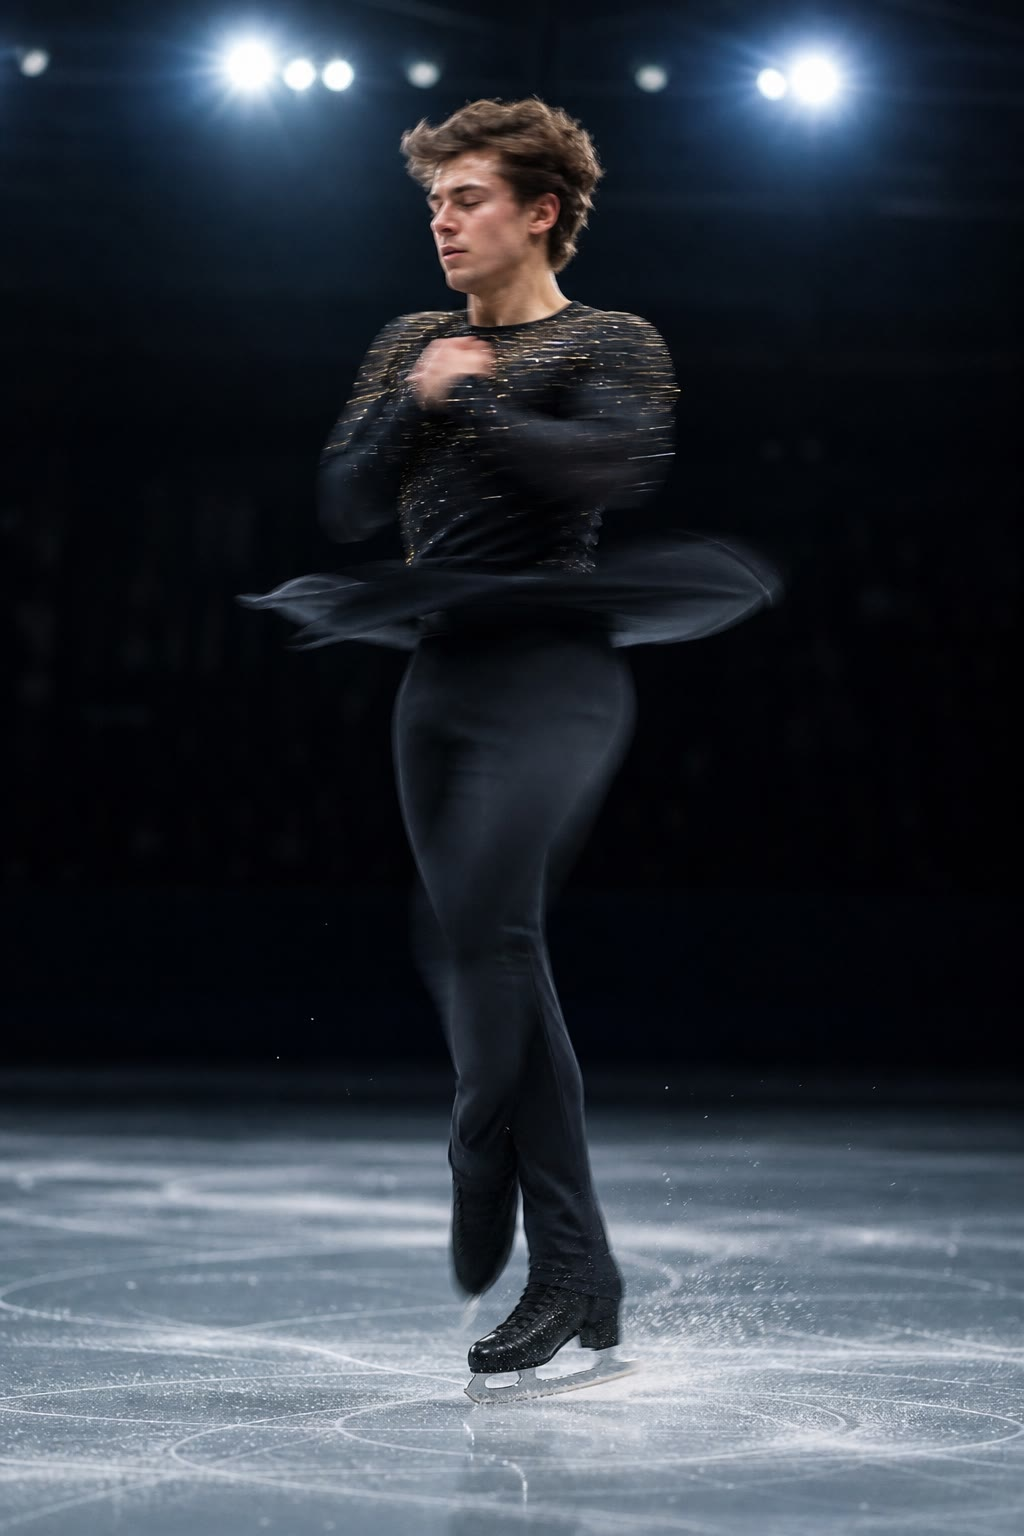
\includegraphics[width=0.34\linewidth]{images/book3/ai/b3-15-figure-skater-spin.jpg}

{\small 手臂收回后，滑冰运动员转得更快：若对竖直轴的外\omterm{def:b1:angular-momentum:moment}{力矩}为零，则角\omterm{def:b1:newton-dynamics:conservation}{动量守恒}，\omterm{prop:b1:angular-momentum:inertia}{转动惯量}越小，\omterm{cor:b1:point-kinematics:circular}{角速度}越大。}
\end{omfigure}

\section{力矩}

\begin{definition}[对一点的力矩；对一轴的力矩]\label{def:b1:angular-momentum:moment}
\index{力的力矩}\index{力矩}\index{力臂}
对点 $O$ 的\emph{力矩}（或\emph{力矩}）
为力 $\vect F$ 作用于 $M$ 点时的矢量
\[
\vect{\mathcal M}_O(\vect F) = \vect{OM}\wedge\vect F \qquad (\unit{N.m}),
\]
它垂直于 $\vect{OM}$ 与 $\vect F$ 所在的平面，
其模为 $OM\cdot F\sin\alpha = F\,d$，其中 $d$ ——即\emph{力臂}——是 $O$ 到
$\vect F$ 作用线的距离。对有向轴 $\Delta$
（单位矢量为 $\vect e_\Delta$，过 $O$）的力矩为标量
$\mathcal M_\Delta = \vect{\mathcal M}_O\cdot\vect e_\Delta$，它与 $O$ 在 $\Delta$ 上的取法无关；
若 $\vect F$ 与 $\Delta$ 平行或与之相交，则该力矩为零。
作用线不同的两个大小相等、方向相反的力
构成一个\emph{力偶}，其力矩
$\vect F\wedge\vect{AB}$ 对任一点都相同。
\end{definition}

\begin{example}[门]\label{ex:b1:angular-momentum:door}
在距合页 \qty{0.80}{m} 处垂直于门施加 \qty{20}{N} 的推力，
其对合页轴的\omterm{def:b1:angular-momentum:moment}{力矩}为 $\qty{16}{N.m}$；同一推力作用于距合页 \qty{0.10}{m} 处，
\omterm{def:b1:angular-momentum:moment}{力矩}为 \qty{2}{N.m}；沿门的方向施力（作用线过合页）时，
\omterm{def:b1:angular-momentum:moment}{力矩}为零。合页的反作用力与该轴相交，
对该轴无\omterm{def:b1:angular-momentum:moment}{力矩}，这正是该轴自然成为取矩中心的
原因。
\end{example}

\begin{omfigure}
\begin{tikzpicture}[font=\small, x=1cm, y=1cm]
  \fill (0,0) circle (1.6pt) node[below left] {$O$};
  \coordinate (M) at (3.2,1.4);
  \fill[omThm] (M) circle (1.6pt); \node[above left] at (M) {$M$};
  \draw[-Stealth, omExo] (0,0) -- (M) node[midway, above, sloped] {$\vect{OM}$};
  \draw[-Stealth, omDef, very thick] (M) -- ++(1.2,1.9) node[right] {$\vect F$};
  \draw[omDef!60, dashed] ($(M)+(-1.82,-2.87)$) -- ($(M)+(1.9,3.0)$);
  % lever arm: perpendicular from O to the line of action (direction (1.2,1.9) normalized (0.534,0.845)); foot = M + t*(dir) with t = -(OM . dir)
  \coordinate (H) at ($(M)+(-0.534*2.892,-0.845*2.892)$);
  \draw[omProp, thick] (0,0) -- (H) node[midway, below right, xshift=3pt] {$d$};
  \draw ($(H)+(0.13,0.2)$) -- ($(H)+(0.13-0.17,0.2+0.1)$) -- ($(H)+(-0.17,0.1)$);
  \draw[dashed] (M) -- ++(23.6:1.3);
  \draw ($(M)+(23.6:0.9)$) arc (23.6:57.7:0.9); \node at ($(M)+(40.5:1.15)$) {$\alpha$};
  \node[omProp, font=\footnotesize] at (4.6,-0.5) {$\abs{\vect{\mathcal M}_O} = F\,d = OM\cdot F\sin\alpha$};
\end{tikzpicture}

{\small $\vect F$ 对 $O$ 的\omterm{def:b1:angular-momentum:moment}{力矩}：叉积
$\vect{OM}\wedge\vect F$，其模为 $F\,d$，$d$ 为 $O$
到作用线的距离（即\omterm{def:b1:angular-momentum:moment}{力臂}），方向垂直于图面，
此处指向读者。}
\end{omfigure}

\section{质点的角动量}

\begin{definition}[角动量]\label{def:b1:angular-momentum:L}
\index{角动量}
对 $O$ 的\emph{角动量}，指质量为 $m$ 的质点
位于点 $M$、速度为 $\vect v$ 时，其为：
\[
\vect L_O = \vect{OM}\wedge m\vect v \qquad (\unit{kg.m^2/s}),
\]
对轴 $\Delta$（过 $O$），$L_\Delta = \vect L_O\cdot\vect e_\Delta$。
若运动位于垂直于 $\Delta$ 的平面内，则以轴为极点取\omterm{def:b1:point-kinematics:cylindrical}{极坐标}，
$L_\Delta = mr^2\dot\theta$；对半径为 $R$ 的\omterm{cor:b1:point-kinematics:circular}{圆周运动}，
$L_\Delta = mR^2\omega = mRv$。
\end{definition}

\begin{proof}
$\vect{OM} = r\vect e_r$, $\vect v = \dot r\vect e_r + r\dot\theta\vect e_\theta$:
$\vect{OM}\wedge m\vect v = mr^2\dot\theta\,\vect e_r\wedge\vect e_\theta = mr^2\dot\theta\,\vect e_z$.
\end{proof}

\begin{theorem}[角动量定理]\label{thm:b1:angular-momentum:theorem}
\index{角动量定理}
在惯性系中，对该系中固定的点 $O$，
\[
\frac{\dd\vect L_O}{\dd t} = \sum\vect{\mathcal M}_O(\vect F_i),
\qquad
\frac{\dd L_\Delta}{\dd t} = \sum\mathcal M_\Delta(\vect F_i)
\]
对固定轴 $\Delta$ 成立；若对 $O$ 的总\omterm{def:b1:angular-momentum:moment}{力矩}为零，
则 $\vect L_O$ 守恒。
\end{theorem}

\begin{proof}
$\dd(\vect{OM}\wedge m\vect v)/\dd t = \vect v\wedge m\vect v + \vect{OM}\wedge m\vect a
= \vect 0 + \vect{OM}\wedge\sum\vect F_i$，由牛顿第二定律
（$O$ 固定，故 $\dd\vect{OM}/\dd t = \vect v$）。在 $\vect e_\Delta$ 上投影即得。
\end{proof}

\begin{corollary}[有心力：平面运动与面积定律]\label{cor:b1:angular-momentum:central}
\index{有心力}\index{面积定律}\index{面积速度}
仅受\emph{有心力}作用的质点（力总沿
$\vect{OM}$ 方向，指向或背离定点 $O$）保持 $\vect L_O$ 不变。其运动位于过 $O$
且垂直于 $\vect L_O$ 的平面内，在该平面内 $r^2\dot\theta = C$
（常量）。位矢 $\vect{OM}$ 以恒定的
\emph{\omterm{cor:b1:angular-momentum:central}{面积速度}}扫过面积，
其值为
\[
\frac{\dd A}{\dd t} = \frac12 r^2\dot\theta = \frac{L_O}{2m} = \frac{C}{2} .
\]
\end{corollary}

\begin{proof}
$\vect{OM}\wedge\vect F = \vect 0$（$\vect F \parallel \vect{OM}$），故 $\vect L_O$
不变。$\vect{OM}\perp\vect L_O$ 恒成立，因此运动位于一个平面内；$L_O =
mr^2\dot\theta$ 为常量。在 $\dd t$ 内扫过的面积是
以 $\vect{OM}$ 和 $\vect v\dd t$ 为两边的三角形：$\dd A = \tfrac12\abs{\vect{OM}
\wedge\vect v}\dd t = \tfrac12 r^2\dot\theta\,\dd t$。
\end{proof}

\begin{omfigure}
\begin{tikzpicture}[font=\small, x=1cm, y=1cm]
  \fill (0,0) circle (1.8pt) node[below left] {$O$};
  % ellipse orbit with focus at O: a=3, e=0.6 -> c=1.8 ; center at (-1.8,0); b=2.4
  \draw[omDef, thick] (-1.8,0) ellipse (3 and 2.4);
  % sector near perihelion (right): angles from focus; parametrize points on ellipse by param t: (-1.8+3cos t, 2.4 sin t)
  \fill[omThm!25] (0,0) -- (1.2,0) -- ({-1.8+3*cos(20)},{2.4*sin(20)}) -- ({-1.8+3*cos(10)},{2.4*sin(10)}) -- cycle;
  \draw[omThm] (0,0) -- (1.2,0); \draw[omThm] (0,0) -- ({-1.8+3*cos(20)},{2.4*sin(20)});
  % sector near aphelion (left): same area: wider angle
  \fill[omThm!25] (0,0) -- ({-1.8+3*cos(150)},{2.4*sin(150)}) -- ({-1.8+3*cos(163)},{2.4*sin(163)}) -- ({-1.8+3*cos(176)},{2.4*sin(176)}) -- ({-1.8+3*cos(189)},{2.4*sin(189)}) -- cycle;
  \draw[omThm] (0,0) -- ({-1.8+3*cos(150)},{2.4*sin(150)}); \draw[omThm] (0,0) -- ({-1.8+3*cos(189)},{2.4*sin(189)});
  \node[omThm, font=\footnotesize] at (1.0,0.55) {$\dd A$};
  \node[omThm, font=\footnotesize] at (-3.6,0.55) {$\dd A$};
  \draw[-Stealth, omExo, thick] ({-1.8+3*cos(20)},{2.4*sin(20)}) -- ++(-0.5,0.7) node[above] {$\vect v$ （快）};
  \draw[-Stealth, omExo, thick] ({-1.8+3*cos(170)},{2.4*sin(170)}) -- ++(-0.15,-0.45) node[left] {$\vect v$ （慢）};
\end{tikzpicture}

{\small 有心力的面积定律：相等时间内，从中心 $O$ 出发的位矢
扫过相等的面积，因此质点靠近 $O$ 时运动快，远离时运动慢
——这就是开普勒第二定律，仅由 $\vect L_O$ 守恒即可导出，
与力的
具体形式无关。}
\end{omfigure}

\begin{example}[用力矩求单摆]\label{ex:b1:angular-momentum:pendulum}
\omterm{ex:b1:newton-dynamics:pendulum}{单摆}，取过支点且垂直于摆动平面的轴 $\Delta$：
$L_\Delta = m\ell^2\dot\theta$；张力与轴相交（\omterm{def:b1:angular-momentum:moment}{力矩}为零），
重\omterm{def:b1:angular-momentum:moment}{力的力矩}为 $-mg\ell\sin\theta$（\omterm{def:b1:angular-momentum:moment}{力臂}
$\ell\sin\theta$，起恢复作用）。由定理可得 $m\ell^2\ddot\theta =
-mg\ell\sin\theta$，即\cref{ex:b1:newton-dynamics:pendulum}中的方程，
且无需写出张力——这正是\omterm{def:b1:angular-momentum:moment}{力矩}方法的主要优点：
通过轴的力不出现在方程中。
\end{example}

\begin{example}[把小滑块向内拉]\label{ex:b1:angular-momentum:puck}
一小滑块在无摩擦的冰面上沿圆周滑动，由穿过中心小孔的绳子拉住，
绳子被拉动，使半径减半。
张力指向中心，$L = mr^2\omega$ 守恒，故 $\omega$
变为原来的 $4$ 倍，速率 $r\omega$ 变为原来的 $2$ 倍，\omterm{thm:b1:work-and-energy:ke}{动能}变为原来的 $4$ 倍
——多出的能量即为拉力所做的功，滑块在整个
向内运动过程中都在抵抗拉力。滑冰者手臂的运动遵循同样的物理规律，只是质量分布不同（
见\cref{exo:b1:angular-momentum:4}）。
\end{example}

\section{质点系与定轴转动}

\begin{theorem}[质点系的角动量]\label{thm:b1:angular-momentum:system}
\index{角动量!质点系的}
对质点系，取 $\vect L_O = \sum_i\vect{OM_i}\wedge m_i\vect v_i$，
且 $O$ 在\omterm{thm:b1:newton-dynamics:laws}{惯性参考系}中固定，则
\[
\frac{\dd\vect L_O}{\dd t} = \sum\vect{\mathcal M}_O(\vect F_{\mathrm{ext}}):
\]
只有\emph{外}\omterm{def:b1:angular-momentum:moment}{力的力矩}有贡献；内力
它们沿质点间连线满足\omterm{thm:b1:newton-dynamics:laws}{作用与反作用}定律，
不作贡献。
\end{theorem}

\begin{proof}
对各质点应用质点定理并求和。对一对内力，$\vect{OM_i}\wedge\vect F_{j\to i}
+ \vect{OM_j}\wedge\vect F_{i\to j} = (\vect{OM_i} - \vect{OM_j})\wedge\vect F_{j\to i}
= \vect{M_jM_i}\wedge\vect F_{j\to i} = \vect 0$，因为力沿
$\vect{M_jM_i}$ 方向。
\end{proof}

\begin{proposition}[刚性定轴转动]\label{prop:b1:angular-momentum:inertia}
\index{转动惯量}
若各质点的距离 $r_i$ 相对于轴 $\Delta$ 保持不变，且都
以相同的\omterm{cor:b1:point-kinematics:circular}{角速度} $\omega$ 绕该轴转动（刚性转动），则
\[
L_\Delta = J_\Delta\,\omega, \qquad J_\Delta = \sum_i m_ir_i^2, \qquad
E_k = \tfrac12 J_\Delta\omega^2,
\]
其中 $J_\Delta$ 为关于 $\Delta$ 的\emph{\omterm{prop:b1:angular-momentum:inertia}{转动惯量}}，
定理写为 $J_\Delta\dot\omega = \sum\mathcal M_\Delta(\vect F_{\mathrm{ext}})$。
\end{proposition}

\begin{proof}
每个质点贡献 $m_ir_i^2\omega$ 于 $L_\Delta$，
贡献 $\tfrac12 m_i(r_i\omega)^2$ 于 $E_k$。在\cref{ch:b1:systems-of-points}
中，此结论可推广到连续固体。
\end{proof}

\begin{example}[滑冰者]\label{ex:b1:angular-momentum:skater}
双臂伸开时，滑冰者身体的\omterm{prop:b1:angular-momentum:inertia}{转动惯量}约为 $J \approx \qty{4}{kg.m^2}$，加上两只
\qty{3}{kg}、位于 \qty{0.8}{m} 处的手臂：$J_1 = 4 + 2 \times 3 \times 0.64 =
\qty{7.8}{kg.m^2}$。双臂收回（\qty{0.2}{m}）时：$J_2 = \qty{4.2}{kg.m^2}$。
冰面的反作用力和重力对竖直轴的\omterm{def:b1:angular-momentum:moment}{力矩}均为零，
故 $J\omega$ 守恒，转速增大为原来的 $J_1/J_2 = 1.85$ 倍
——从每秒 $2$ 转增至每秒 $3.7$ 转——而\omterm{thm:b1:work-and-energy:ke}{动能}
按同一倍数增大，所需能量由肌肉收拢手臂时做功提供。
\end{example}

\begin{omfigure}
\begin{tikzpicture}[font=\small, x=1cm, y=1cm]
  \draw[-Stealth, thick] (0,-0.6) -- (0,3.4) node[above] {$\Delta$};
  \draw[omDef!40, dashed] (0,1.2) ellipse (2.2 and 0.55);
  \draw[omDef!40, dashed] (0,2.2) ellipse (1.3 and 0.33);
  \fill[omThm] (2.2,1.2) circle (2.2pt) node[right] {$m_1$};
  \fill[omThm] (-1.3,2.2) circle (2.2pt) node[left] {$m_2$};
  \fill[omThm] (1.1,0.73) circle (2.2pt) node[below right] {$m_3$};
  \draw[omExo] (0,1.2) -- (2.2,1.2) node[midway, above] {$r_1$};
  \draw[omExo] (0,2.2) -- (-1.3,2.2) node[midway, above] {$r_2$};
  \draw[-Stealth, omDef, thick] (2.2,1.2) -- ++(0,-0.0) ++(0,0) -- ++(-0.1,-0.5);
  \draw[-Stealth, omDef, thick] (-1.3,2.2) -- ++(0.05,0.5);
  \draw[-Stealth, omProp, thick] (0.7,3.0) arc (80:10:0.7) node[right] {$\omega$};
  \node[font=\footnotesize] at (3.8,2.6) {$L_\Delta = \Big(\sum m_ir_i^2\Big)\omega$};
\end{tikzpicture}

{\small 绕同一轴刚性转动的质点：每个质点都在自身的圆周上，以共同的
$\omega$ 转动，对该轴\omterm{def:b1:angular-momentum:L}{角动量}的贡献为 $m_ir_i^2\omega$。
离轴越远的质量，其贡献按距离的平方计
——正是滑冰者伸开的双臂。}
\end{omfigure}

\begin{remark}[静力学]\label{rem:b1:angular-momentum:statics}
\index{固体的平衡}
静止的固体有 $\vect L_O = \vect 0$ 恒定：外力
的合力须为零，\emph{且}对任一点的总\omterm{def:b1:angular-momentum:moment}{力矩}也须为零。
第二个条件就是天平、跷跷板和撬棍的杠杆定律：
离支点较远的小力，
可与离支点较近的大力平衡。
\end{remark}

\section{练习}

\begin{exercise}[$\star$]\label{exo:b1:angular-momentum:1}
作用于扳手上、距螺母 \qty{0.30}{m} 处的 \qty{50}{N} 力，求其\omterm{def:b1:angular-momentum:moment}{力矩}：
分别在力与手柄垂直、与手柄成 $60^\circ$ 及沿手柄方向时
求出\omterm{def:b1:angular-momentum:moment}{力矩}。
\end{exercise}

\begin{exercise}[$\star$]\label{exo:b1:angular-momentum:2}
求地球绕太阳的\omterm{def:b1:angular-momentum:L}{角动量}（轨道视为圆形，
$r = \qty{1.50e11}{m}$, $v = \qty{29.8}{km/s}$, $m = \qty{5.97e24}{kg}$),
并求其\omterm{cor:b1:angular-momentum:central}{面积速度}。
\end{exercise}

\begin{exercise}[$\star$]\label{exo:b1:angular-momentum:3}
一个圆锥摆（绳长 \qty{1.0}{m}，与竖直方向成 $30^\circ$，
见\cref{exo:b1:newton-dynamics:9}）。求对过支点竖直轴的单位质量\omterm{def:b1:angular-momentum:L}{角动量} $L$，
并说明为何虽有绳的张力和重力作用，
该\omterm{def:b1:angular-momentum:L}{角动量}仍然守恒。
\end{exercise}

\begin{exercise}[$\star$]\label{exo:b1:angular-momentum:4}
滑冰者躯干对自转轴的\omterm{prop:b1:angular-momentum:inertia}{转动惯量}为 $J = \qty{4.0}{kg.m^2}$，
每条手臂（\qty{3.0}{kg}）先视为位于 \qty{0.80}{m} 处的质点，
再视为位于 \qty{0.20}{m} 处的质点。求收回手臂后的
转速（初始为每秒 \qty{2.0}{} 转）及\omterm{thm:b1:work-and-energy:ke}{动能}之比，
多出的能量来自何处？
\end{exercise}

\begin{exercise}[$\star\star$]\label{exo:b1:angular-momentum:5}
由对支点轴的\omterm{def:b1:angular-momentum:L}{角动量}定理导出\omterm{ex:b1:newton-dynamics:pendulum}{单摆}方程 $\ell\ddot\theta + g\sin\theta = 0$，
并写出
各\omterm{def:b1:angular-momentum:moment}{力的力矩}。
\end{exercise}

\begin{exercise}[$\star\star$]\label{exo:b1:angular-momentum:6}
地球到太阳的距离在 \qty{1.471e11}{m}（近日点）
与 \qty{1.521e11}{m}（远日点）之间变化。利用面积定律，求两点速率之比，
已知平均速率为 \qty{29.8}{km/s}，
并求两点的速率。
\end{exercise}

\begin{exercise}[$\star\star$]\label{exo:b1:angular-momentum:7}
一个质量为 \qty{0.20}{kg} 的冰球，以 \qty{2.0}{m/s} 的速率绕圈运动，系于穿过小孔、长 \qty{0.50}{m} 的绳上；
拉绳使半径缩小至 \qty{0.25}{m}。
求新的速率和\omterm{cor:b1:point-kinematics:circular}{角速度}，拉绳前后的\omterm{thm:b1:work-and-energy:ke}{动能}，以及
拉力所做的功。为何此处的张力能够做功？
\end{exercise}

\begin{exercise}[$\star\star$]\label{exo:b1:angular-momentum:8}
一块质量为 \qty{20}{kg}、长 \qty{4.0}{m} 的均匀木板，搁在
距左端 \qty{1.5}{m} 处的支点上，质量为 \qty{30}{kg} 的孩子坐在
左端。质量为 \qty{45}{kg} 的孩子应坐在何处才能平衡？
支点承受的是什么？
\end{exercise}

\begin{exercise}[$\star\star$]\label{exo:b1:angular-momentum:9}
阿特伍德机（$m_1 = \qty{2.0}{kg}$，$m_2 = \qty{1.0}{kg}$）跨过
半径为 \qty{0.10}{m}、\omterm{prop:b1:angular-momentum:inertia}{转动惯量}为 \qty{0.010}{kg.m^2} 的滑轮，绳在轮上不打滑。
利用滑轮的\omterm{def:b1:angular-momentum:L}{角动量}定理与质量块的牛顿定律，
求加速度及两段绳中的张力，
并与无质量滑轮的情形作比较。
\end{exercise}

\begin{exercise}[$\star\star\star$]\label{exo:b1:angular-momentum:10}
一颗彗星经过近日点时，距太阳 \qty{0.50}{AU}，
速率为 \qty{40}{km/s}。当其距太阳 \qty{10}{AU} 时，求其速度
垂直于径矢的分量为多少？面积定律
能否给出其完整速率？
\end{exercise}

\begin{exercise}[$\star\star\star$]\label{exo:b1:angular-momentum:11}
一颗与太阳相似的恒星（$R = \qty{7.0e8}{m}$，自转周期为 \qty{25}{d}），
坍缩成半径为 \qty{10}{km} 的中子星，并保持其质量不变，
\omterm{def:b1:angular-momentum:L}{角动量}亦不变（$J \propto MR^2$）。求新周期与赤道速率。
后者对该假设说明了什么？
\end{exercise}

\begin{exercise}[$\star\star\star$]\label{exo:b1:angular-momentum:12}
一个小珠无摩擦地沿一根直杆滑动，直杆在水平面内
以恒定 $\omega$ 绕过其一端的竖直轴转动。写出小珠的 $L_z$，
并证明它\emph{不}守恒，
求直杆必须施加的\omterm{def:b1:angular-momentum:moment}{力矩}，并由此推出
直杆对小珠的横向反作用力。
\end{exercise}

\section{问题：为什么月球在远离}

\begin{problem}[{周末问题——月球在地球上引起的潮汐把地球向前拉、又把地球拉回：
角动量如何从地球的自转流入月球轨道，
一厘米一厘米地进行，
以及能量去向何处}]
\label{pb:b1:angular-momentum:1}
数据：$G = \qty{6.67e-11}{SI}$；地球 $M = \qty{5.97e24}{kg}$，$R =
\qty{6.37e6}{m}$，自转 $\Omega = 2\pi/(\qty{86164}{s})$，\omterm{prop:b1:angular-momentum:inertia}{转动惯量}
$J = 0.33\,MR^2$；月球 $m = \qty{7.35e22}{kg}$，轨道视为
圆形，$r = \qty{3.84e8}{m}$；月球激光测距测得
$\dd r/\dd t = \qty{3.8}{cm/yr}$；昼长每世纪增加 \qty{2.3}{ms}；
$1$ 世纪 $= \qty{3.16e9}{s}$。

\medskip
\noindent\textbf{第一部分——\omterm{def:b1:angular-momentum:L}{角动量}。}
\begin{enumerate}
  \item 由牛顿定律（圆轨道）求月球的轨道\omterm{cor:b1:point-kinematics:circular}{角速度} $\omega$，
        并与恒星月
        \qty{27.3}{d} 进行核对。
  \item 求月球的轨道\omterm{def:b1:angular-momentum:L}{角动量} $L_{\text{轨道}} =
        mr^2\omega$。
  \item 证明对于圆轨道 $L_{\text{轨道}} = m\sqrt{GMr}$，
        由此推出 $\dd L_{\text{轨道}}/\dd r = L_{\text{轨道}}/2r$。
  \item 求地球的自转\omterm{def:b1:angular-momentum:L}{角动量} $L_{\text{自旋}} =
        J\Omega$，并与 $L_{\text{轨道}}$ 比较。
  \item 月球每月自转一周：估算其自转\omterm{def:b1:angular-momentum:L}{角动量}
        （$J_m \approx 0.4\,mR_m^2$，$R_m = \qty{1.74e6}{m}$），
        并说明为何可以忽略。
  \item 地月系统相对其质心受到哪些外\omterm{def:b1:angular-momentum:moment}{力矩}作用？
        论证在较好的近似下，总\omterm{def:b1:angular-momentum:L}{角动量}
        $L = L_{\text{自旋}} + L_{\text{轨道}}$ 守恒。
\end{enumerate}

\medskip
\noindent\textbf{第二部分——潮汐\omterm{def:b1:angular-momentum:moment}{力矩}。}
月球在地球上引起两个水的隆起；由于地球自转快于月球绕行，
摩擦力把隆起拖到地月连线之前，
即超前地月连线一个小角度。
\begin{enumerate}[resume]
  \item 画出地球、超前的隆起与月球的示意图，
        月球对较近隆起的吸引力朝哪个方向作用，
        相对于地球自转方向？
  \item 推断地球自转所受\omterm{def:b1:angular-momentum:moment}{力矩}的符号：
        昼长是变长还是变短？
  \item 由\omterm{thm:b1:newton-dynamics:laws}{作用与反作用}，月球轨道运动受到什么\omterm{def:b1:angular-momentum:moment}{力矩}？
        $L_{\text{轨道}}$ 是增大还是减小？
  \item 由第 3 题，$r$ 是增大还是减小？月球的轨道
        速率 $v = \sqrt{GM/r}$ 呢？
  \item 解释这一表观佯谬：月球被向前推，
        最终却运动得更慢。
  \item 这种交换趋向于怎样的最终状态？
\end{enumerate}

\medskip
\noindent\textbf{第三部分——数值。}
\begin{enumerate}[resume]
  \item 由昼长的增加，求每世纪的相对变化
        $\Delta\Omega/\Omega$。
  \item 推出每世纪 $L_{\text{自旋}}$ 的变化。
  \item 推出每世纪 $L_{\text{轨道}}$ 的变化。
  \item 利用第 3 题，把它换算为 $r$ 每世纪和每年的变化，
        并与激光测距值比较。
  \item 恒星月每世纪增加了多大比例，又增加了多少秒
        （$T \propto r^{3/2}$）？
  \item 求地球自转\omterm{thm:b1:work-and-energy:ke}{动能}每世纪的变化
        （$\Delta E = L_{\text{自旋}}\Delta\Omega$，
        取一阶近似）。
  \item 求月球的轨道\omterm{thm:b1:work-and-energy:em}{机械能}
        $E_{\text{轨道}} = -GMm/2r$ 每世纪的变化。
\end{enumerate}

\medskip
\noindent\textbf{第四部分——能量。}
\begin{enumerate}[resume]
  \item 证明地球损失的能量多于月球获得的能量，
        并求每世纪的差值及相应的功率，
        它去了哪里？
  \item 将该功率与人类约
        \qty{18}{TW} 的能耗相比较，并与地球
        内部热流约 \qty{47}{TW} 相比较。
  \item 在第 12 题的最终状态中，日与月相等：
        $\Omega = \omega = \sqrt{GM/r^3}$。写出 $L_{\text{自旋}} + L_{\text{轨道}}$ 守恒，
        验证 $r \approx
        \qty{5.5e8}{m}$ 满足它，并给出共同的周期（以天计）。
  \item 为何该状态实际上永远无法达到？（想一想太阳的
        潮汐。）
  \item 月球已经只向地球展示一个面。用同样的机制加以解释，
        并说明为何这一现象率先发生在月球上。
  \item 用三句话概括：什么守恒，什么被交换，
        什么被耗散。
\end{enumerate}
\end{problem}
